\hypertarget{poly_8h}{
\section{poly.h File Reference}
\label{poly_8h}\index{poly.h@{poly.h}}
}
Declaration of the polynomial class. 

{\tt \#include $<$iostream$>$}\par


Include dependency graph for poly.h:\nopagebreak
\begin{figure}[H]
\begin{center}
\leavevmode
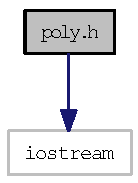
\includegraphics[width=51pt]{poly_8h__incl}
\end{center}
\end{figure}


This graph shows which files directly or indirectly include this file:\nopagebreak
\begin{figure}[H]
\begin{center}
\leavevmode
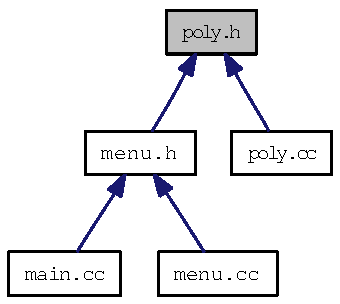
\includegraphics[width=99pt]{poly_8h__dep__incl}
\end{center}
\end{figure}
\subsection*{Classes}
\begin{CompactItemize}
\item 
class \hyperlink{classPolynomial}{Polynomial}
\begin{CompactList}\small\item\em represents the polynomial as a linked list of terms \item\end{CompactList}\item 
class \textbf{Polynomial::term}
\end{CompactItemize}
\subsection*{Functions}
\begin{CompactItemize}
\item 
\hyperlink{classPolynomial}{Polynomial} \hyperlink{poly_8h_a5dcabab23da371f543b0daccb699b9d}{abs} (const \hyperlink{classPolynomial}{Polynomial} \&p)
\item 
\hyperlink{classPolynomial}{Polynomial} \hyperlink{poly_8h_b201f37e58ec35c0d6fc0029ea309a92}{derivative} (const \hyperlink{classPolynomial}{Polynomial} \&p)
\item 
\hyperlink{classPolynomial}{Polynomial} \hyperlink{poly_8h_a512be609af2a7ca60e6ae4fbca63421}{antiderivative} (const \hyperlink{classPolynomial}{Polynomial} \&p)
\end{CompactItemize}


\subsection{Detailed Description}
Declaration of the polynomial class. 

\begin{Desc}
\item[Author:]Daniel Uber \end{Desc}


Definition in file \hyperlink{poly_8h-source}{poly.h}.

\subsection{Function Documentation}
\hypertarget{poly_8h_a5dcabab23da371f543b0daccb699b9d}{
\index{poly.h@{poly.h}!abs@{abs}}
\index{abs@{abs}!poly.h@{poly.h}}
\subsubsection[abs]{\setlength{\rightskip}{0pt plus 5cm}{\bf Polynomial} abs (const {\bf Polynomial} \& {\em p})}}
\label{poly_8h_a5dcabab23da371f543b0daccb699b9d}


\begin{Desc}
\item[Returns:]absolute value of polynomial \end{Desc}


Definition at line 226 of file poly.cc.

References Polynomial::abs().

\begin{Code}\begin{verbatim}226                                    {
227   return p.abs();
228 }
\end{verbatim}
\end{Code}




Here is the call graph for this function:\nopagebreak
\begin{figure}[H]
\begin{center}
\leavevmode
\includegraphics[width=103pt]{poly_8h_a5dcabab23da371f543b0daccb699b9d_cgraph}
\end{center}
\end{figure}
\hypertarget{poly_8h_a512be609af2a7ca60e6ae4fbca63421}{
\index{poly.h@{poly.h}!antiderivative@{antiderivative}}
\index{antiderivative@{antiderivative}!poly.h@{poly.h}}
\subsubsection[antiderivative]{\setlength{\rightskip}{0pt plus 5cm}{\bf Polynomial} antiderivative (const {\bf Polynomial} \& {\em p})}}
\label{poly_8h_a512be609af2a7ca60e6ae4fbca63421}


\begin{Desc}
\item[Returns:]indefinite integral of p with constant 0 \end{Desc}


Definition at line 245 of file poly.cc.

References Polynomial::antiderivative().

\begin{Code}\begin{verbatim}245                                                 {
246   return p.antiderivative();
247 }
\end{verbatim}
\end{Code}




Here is the call graph for this function:\nopagebreak
\begin{figure}[H]
\begin{center}
\leavevmode
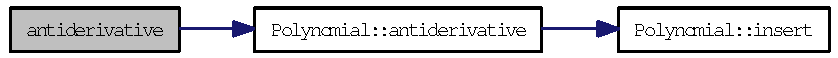
\includegraphics[width=219pt]{poly_8h_a512be609af2a7ca60e6ae4fbca63421_cgraph}
\end{center}
\end{figure}
\hypertarget{poly_8h_b201f37e58ec35c0d6fc0029ea309a92}{
\index{poly.h@{poly.h}!derivative@{derivative}}
\index{derivative@{derivative}!poly.h@{poly.h}}
\subsubsection[derivative]{\setlength{\rightskip}{0pt plus 5cm}{\bf Polynomial} derivative (const {\bf Polynomial} \& {\em p})}}
\label{poly_8h_b201f37e58ec35c0d6fc0029ea309a92}


return polynomial derivative 

Definition at line 209 of file poly.cc.

References Polynomial::derivative().

\begin{Code}\begin{verbatim}209                                            {
210   return p.derivative();
211 }
\end{verbatim}
\end{Code}




Here is the call graph for this function:\nopagebreak
\begin{figure}[H]
\begin{center}
\leavevmode
\includegraphics[width=201pt]{poly_8h_b201f37e58ec35c0d6fc0029ea309a92_cgraph}
\end{center}
\end{figure}
